\chapter{Manual de uso}

Al entrar en la aplicación, lo primero que nos encontramos es la pantalla de inicio de sesión (Figura \ref{fig:man-1}, izquierda). Aquí se introducirán las credenciales del usuario, necesarias en todo momento para acceder a la aplicación. Una vez iniciada la sesión, obtendremos la pantalla principal (Figura \ref{fig:man-1}, derecha). Esta tiene varias secciones las cuales podrían no aparecer todas, en función de permisos de cada usuario. 

\begin{figure}[h!]
    \centering
    
    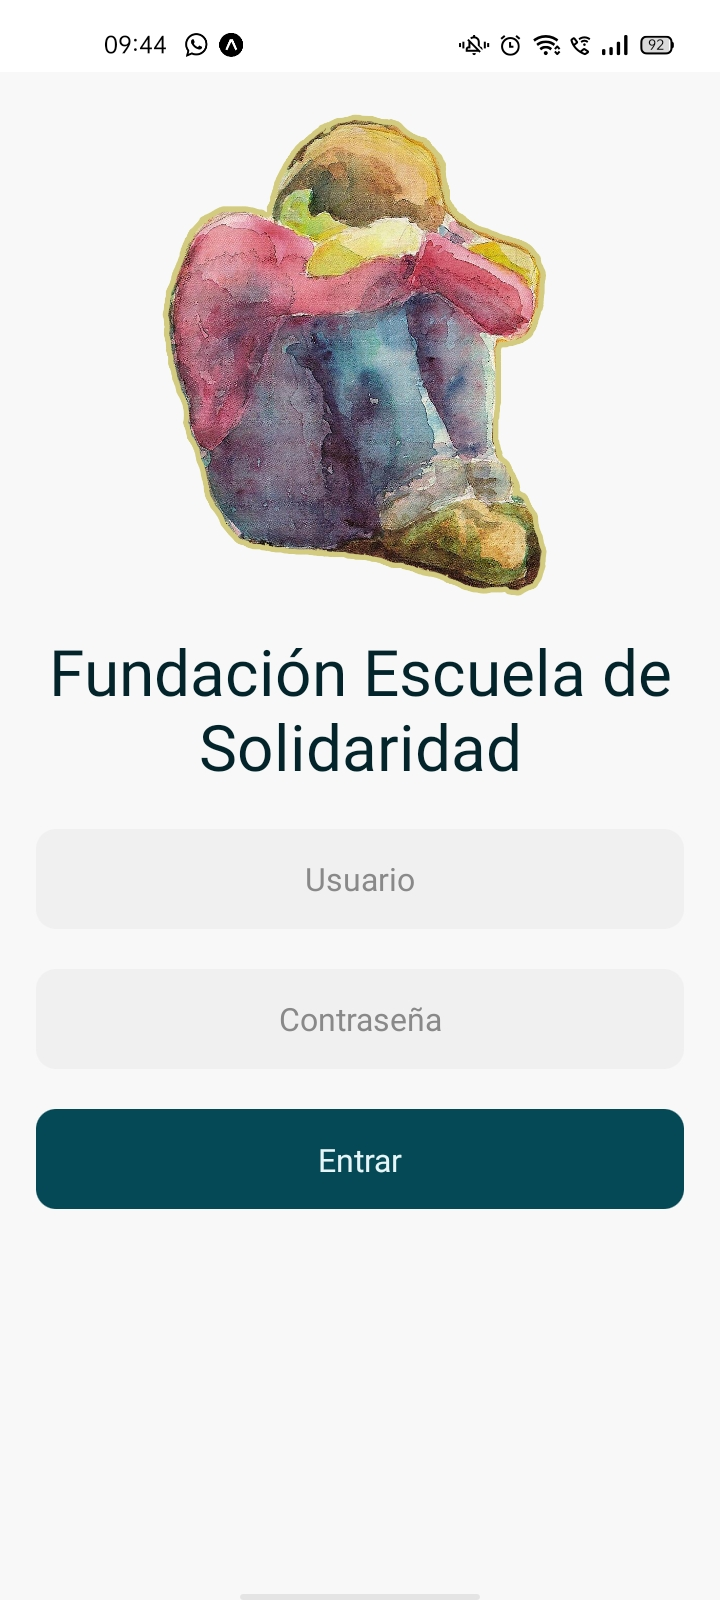
\includegraphics[width=0.30\linewidth]{imagenes/manual_usuario/inicio_sesion.jpg}
    \hspace{0.03\linewidth}
    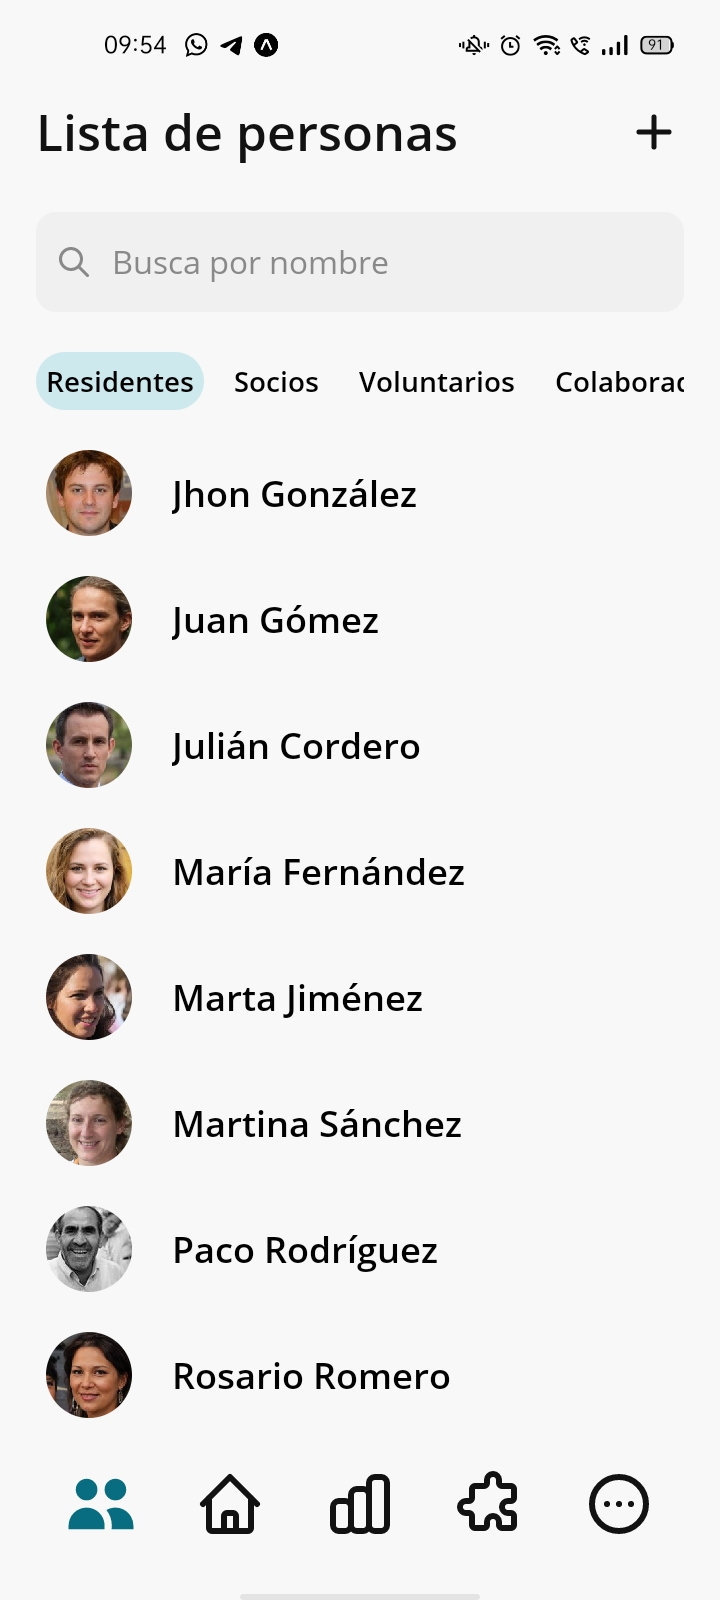
\includegraphics[width=0.30\linewidth]{imagenes/manual_usuario/principal.jpg}
    \hspace{0.03\linewidth}
    \caption{Pantalla de inicio de sesión (izquierda) y pantalla principal (derecha)}
    \label{fig:man-1}

\end{figure}

\subsection{Gestión de personas}

En un usuario con máximos permisos, la primera sección será la de gestión de personas. Aquí nos aparecerá la lista de personas que actualmente hay almacenadas en el sistema y que están dadas de alta. Se podrá acceder a estas según el tipo de cada una. En la parte superior, a la derecha nos encontraremos con el botón para añadir una persona. Al pulsarlo nos llevará a una pantalla de tipo formulario (Figura \ref{fig:man-2}, izquierda) que rellenaremos con los datos de la persona a añadir. 

\begin{figure}[h!]
    \centering
    
    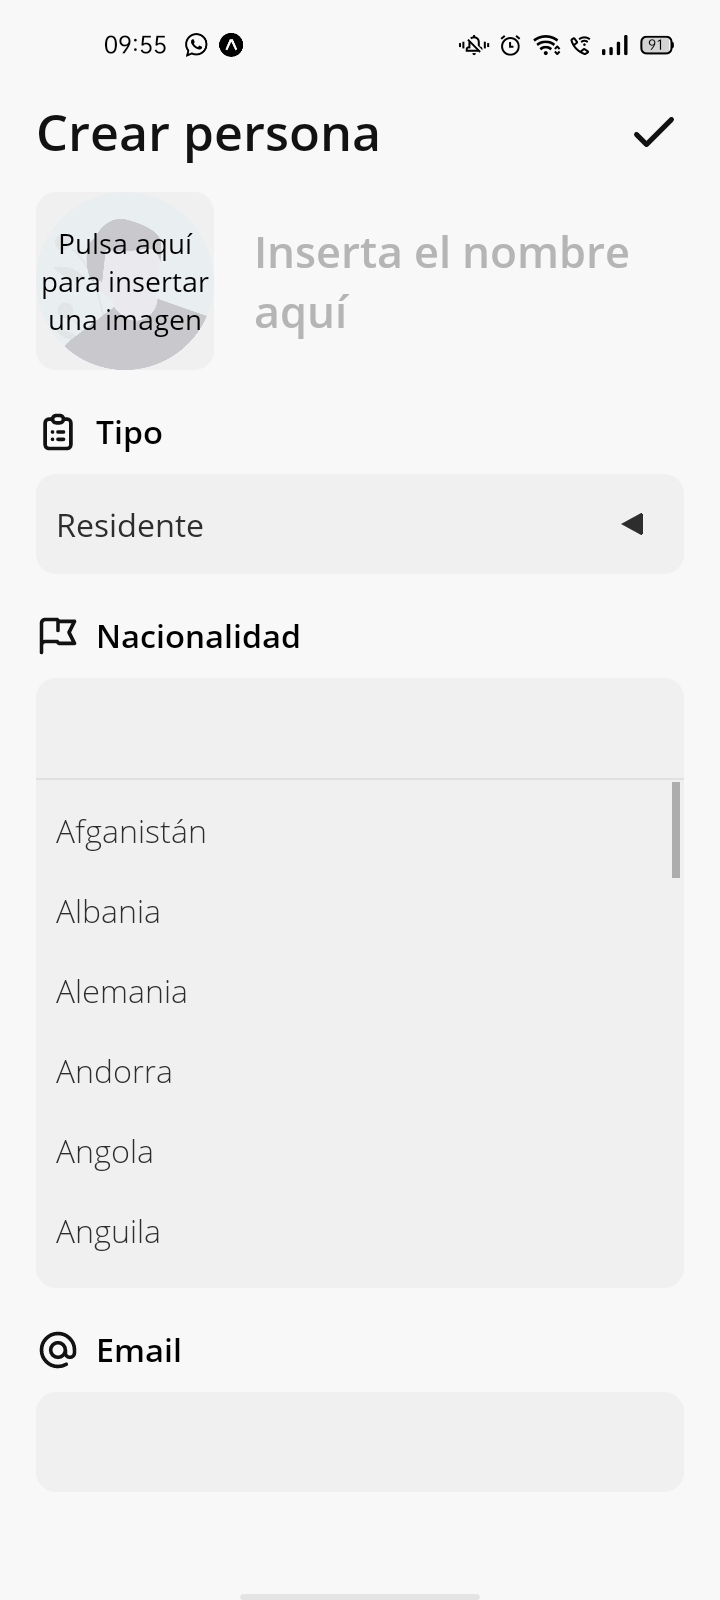
\includegraphics[width=0.30\linewidth]{imagenes/manual_usuario/editar_persona.jpg}
    \hspace{0.03\linewidth}
    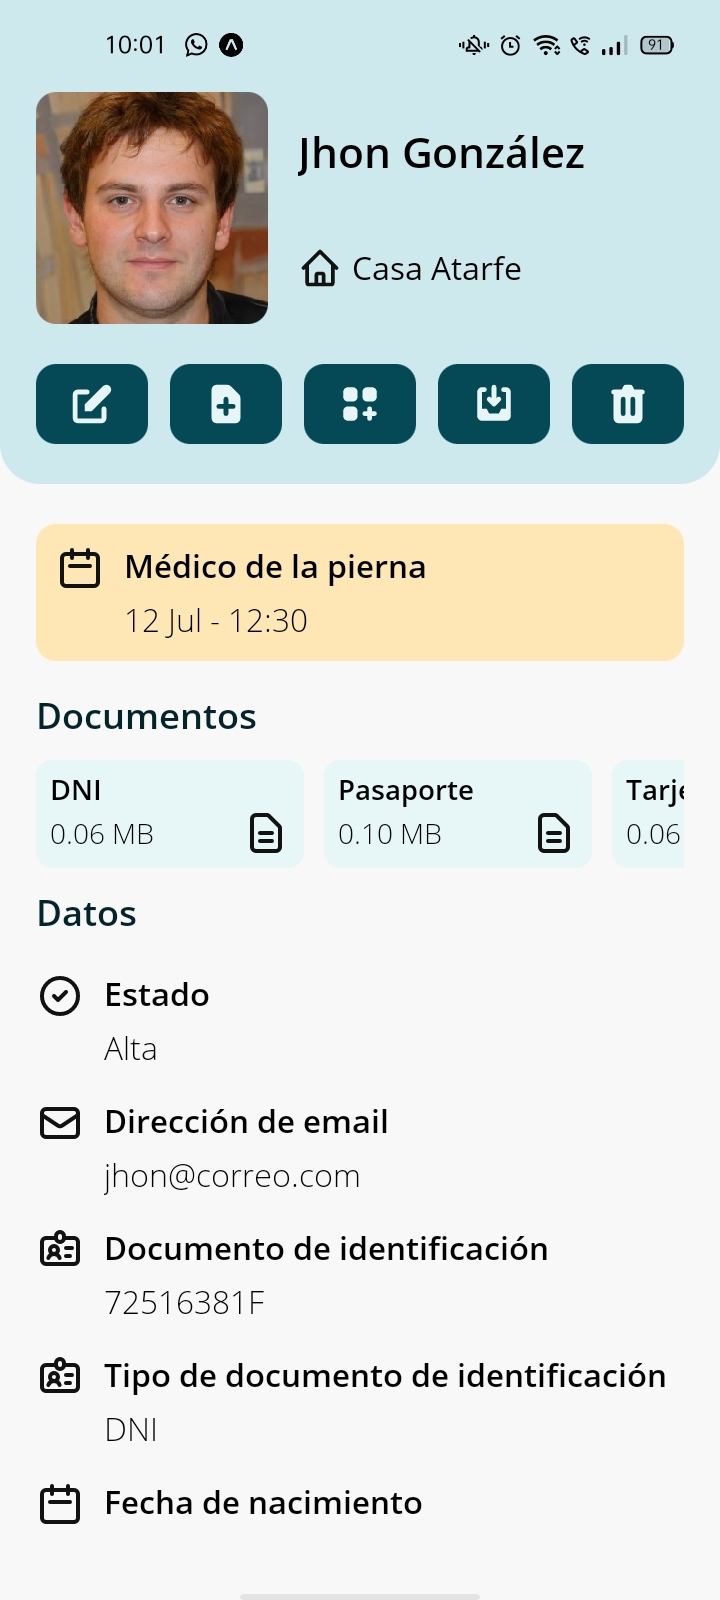
\includegraphics[width=0.30\linewidth]{imagenes/manual_usuario/persona.jpg}
    \hspace{0.03\linewidth}
    \caption{Pantalla para crear una persona (izquierda) y pantalla de una persona (derecha)}
    \label{fig:man-2}

\end{figure}

En la pantalla principal, al pulsar sobre una persona, se navegará hacia una nueva pantalla (Figura \ref{fig:man-2}, derecha) que muestra la información de la persona y las acciones realizables sobre ella. En la parte superior, se muestra su imagen, junto con su nombre y alojamiento si es que tiene uno asignado. Además de esto, se mostrará una fila de botones con los cuales podremos realizar las acciones principales sobre la persona. De izquierda a derecha serán: editar la persona, añadir un nuevo documento, añadir una nueva cita, dar de baja o de alta y eliminar la persona del sistema. 

\begin{itemize}
    \item Editar a la persona: Nos llevará a una pantalla similar a la de crear una nueva persona, con la diferencia de que se cargará la información actual de esa persona.
    \item Añadir un nuevo documento: Aparecerá un ``popup'' que permitirá añadir un nuevo documento cargado desde el propio dispositivo.
    \item Añadir una nueva cita: Aparecerá un ``popup'' que permitirá añadir una nueva cita asociada a la persona.
    \item Dar de baja o alta: Según el estado actual de la persona, se podrá dar de baja o de alta a la persona.
    \item Eliminar: Permitirá eliminar a la persona.
\end{itemize}

En la parte inferior de esta misma pantalla, se mostrarán en el siguiente orden, la próxima cita de la persona, si existe, los documentos de esta y los datos asociados.

\subsection{Gestión de alojamiento}

Para la gestión de alojamiento, tenemos la segunda sección de la aplicación (Figura \ref{fig:man-3}, izquierda). Nos encontraremos con la lista de alojamientos actuales de la fundación junto con la capacidad y ocupación actual de cada uno. 

\begin{figure}[h!]
    \centering
    
    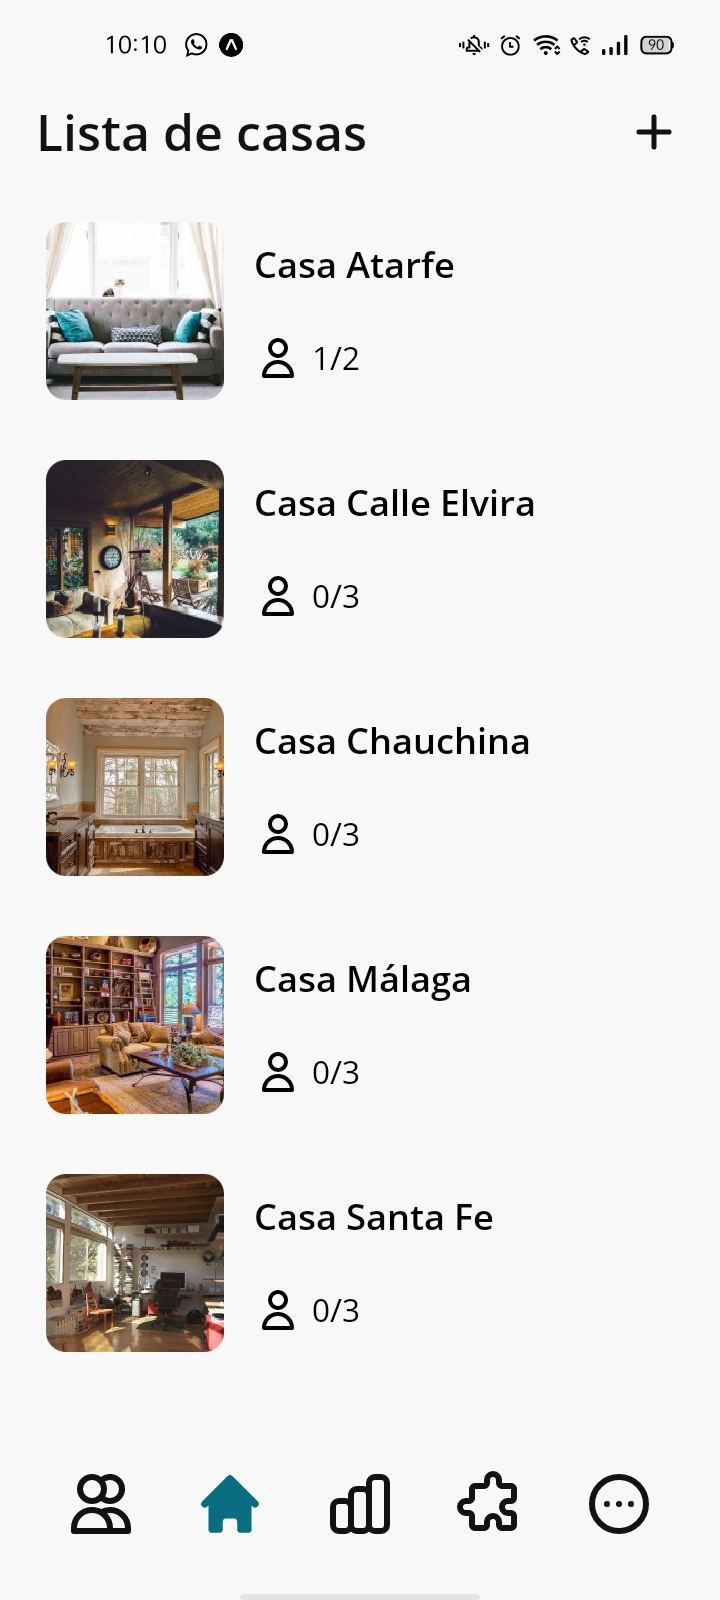
\includegraphics[width=0.30\linewidth]{imagenes/manual_usuario/casas.jpg}
    \hspace{0.03\linewidth}
    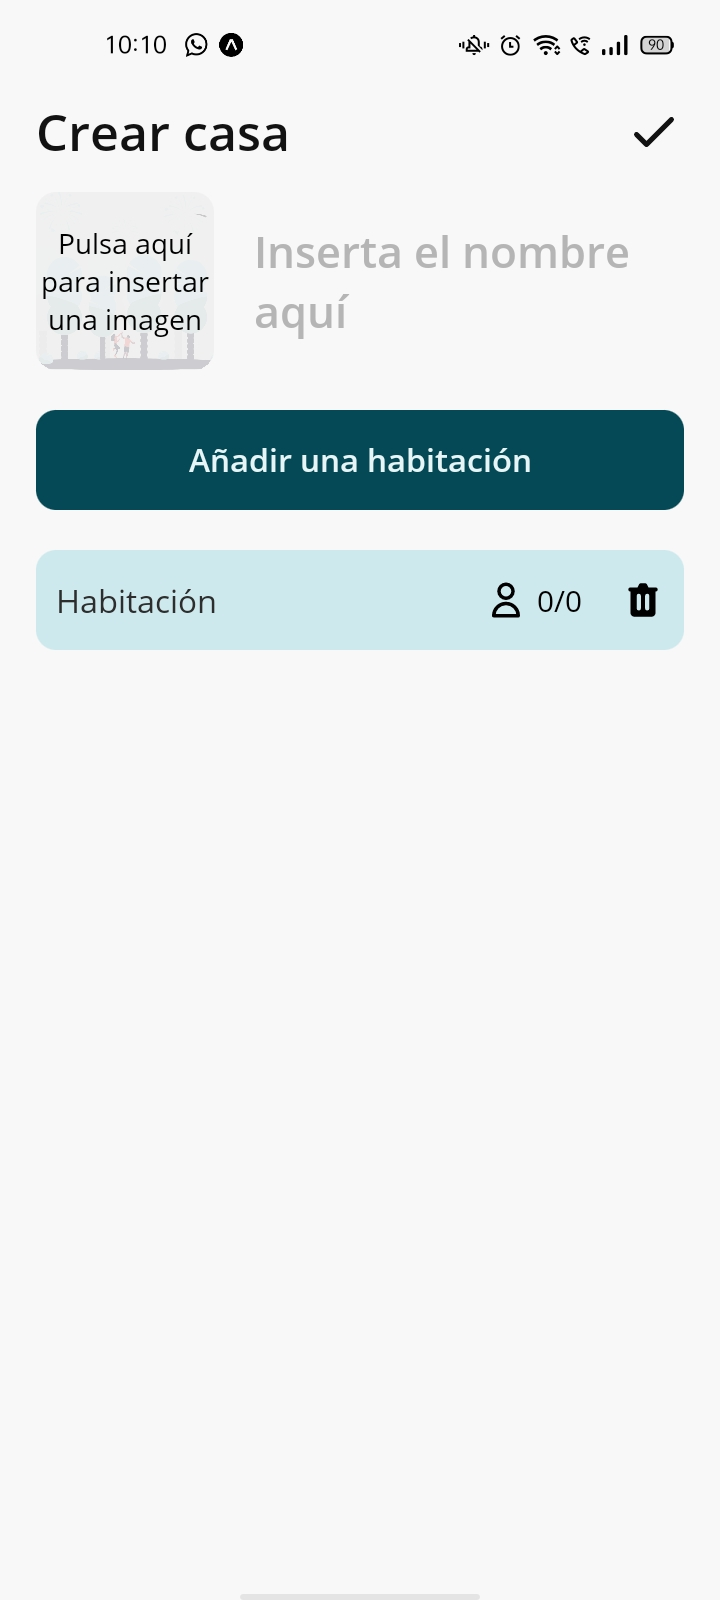
\includegraphics[width=0.30\linewidth]{imagenes/manual_usuario/editar_casa.jpg}
    \hspace{0.03\linewidth}
    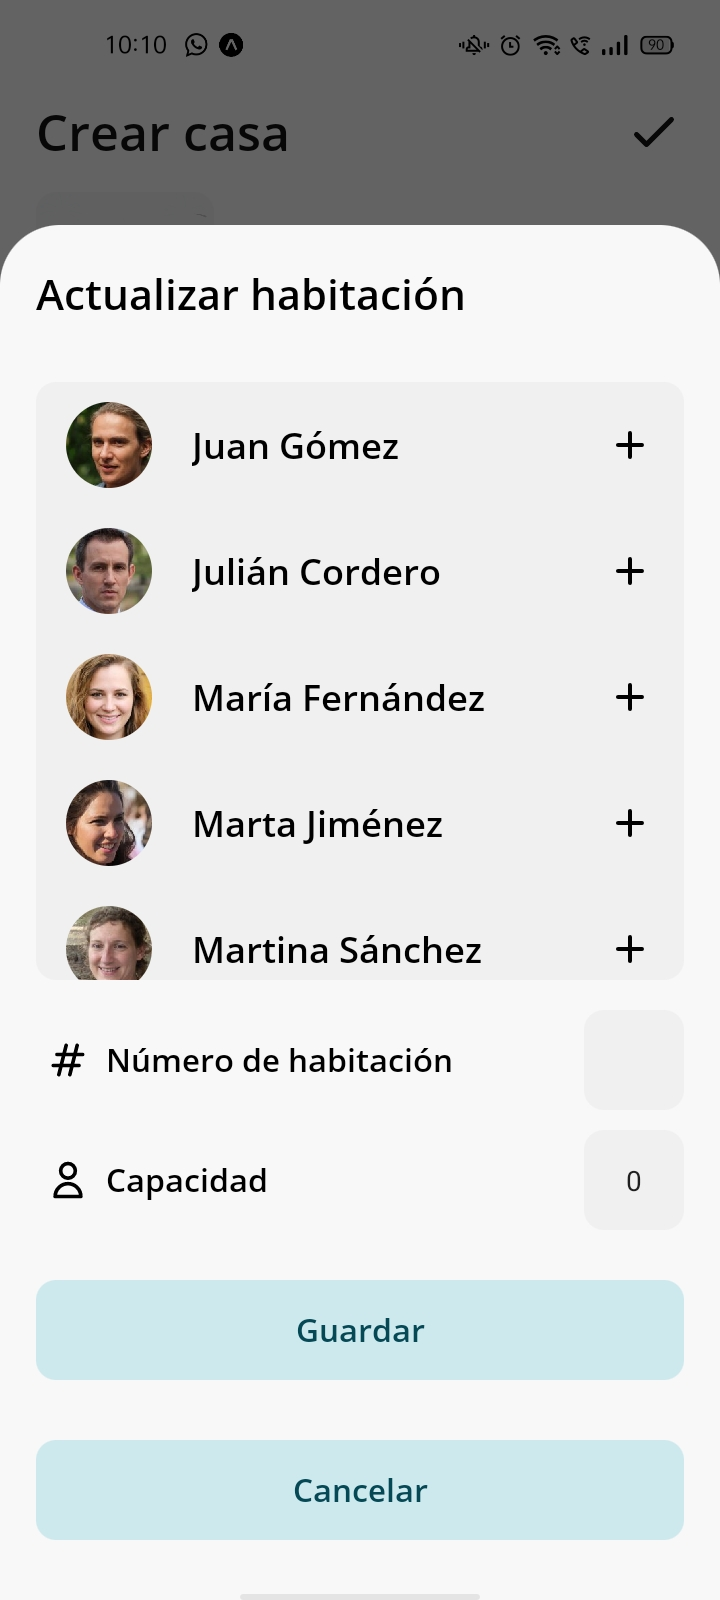
\includegraphics[width=0.30\linewidth]{imagenes/manual_usuario/anadir_habitacion.jpg}
    \caption{Pantalla de casas (izquierda), pantalla para crear una casa (centro) y pantalla para añadir una habitación (derecha)}
    \label{fig:man-3}

\end{figure}

Para añadir una nueva casa, pulsaremos sobre el botón superior. Aquí nos aparecerá un formulario (Figura \ref{fig:man-3}, centro) mediante el cual podremos modificar la información de la casa y añadir o quitar habitaciones. Al pulsar el botón ``Añadir una nueva habitación'', se añadirá un bloque que representará a la habitación. Si pulsamos sobre el se abrirá un popup (Figura \ref{fig:man-3}, derecha) que nos cargará tanto todos los residentes sin alojamiento, como los datos a introducir de la casa. Para añadir o quitar un residente de la habitación pulsaremos sobre él. Podremos confirmar los datos introducidos pulsando en el botón superior derecho.

Si en la lista de alojamientos pulsamos sobre uno de ellos, nos llevará a una pantalla donde podemos ver la información de este (Figura \ref{fig:man-4}, izquierda). Si pulsamos sobre una habitación no aparecerán los residentes de esta. Además aparecerán dos botones de las acciones principales sobre la casa, editarla y eliminarla. La edición vendrá dada por una pantalla similar a la de la creación de una nueva casa. 

\begin{figure}[h!]
    \centering
    
    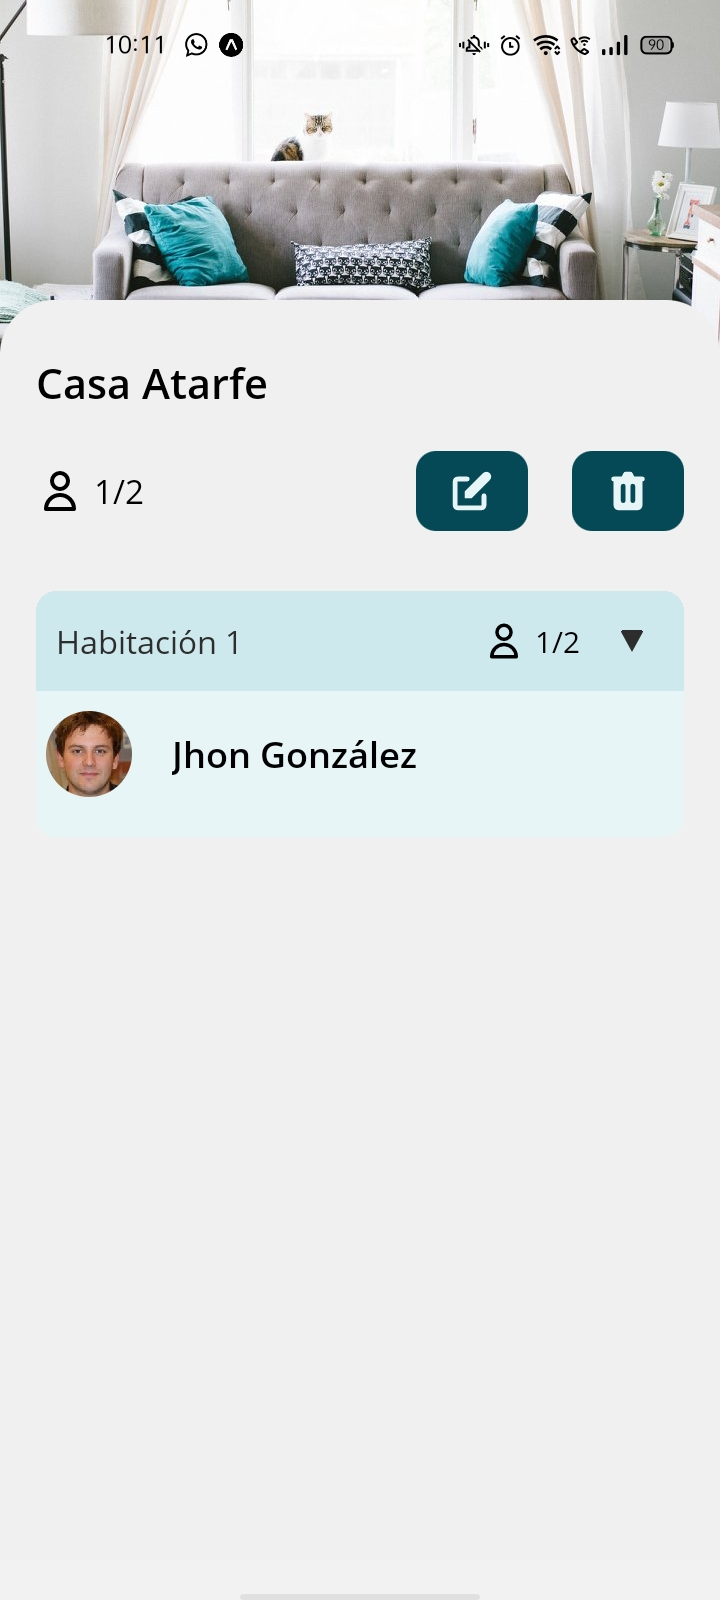
\includegraphics[width=0.30\linewidth]{imagenes/manual_usuario/casa.jpg}
    \hspace{0.03\linewidth}
    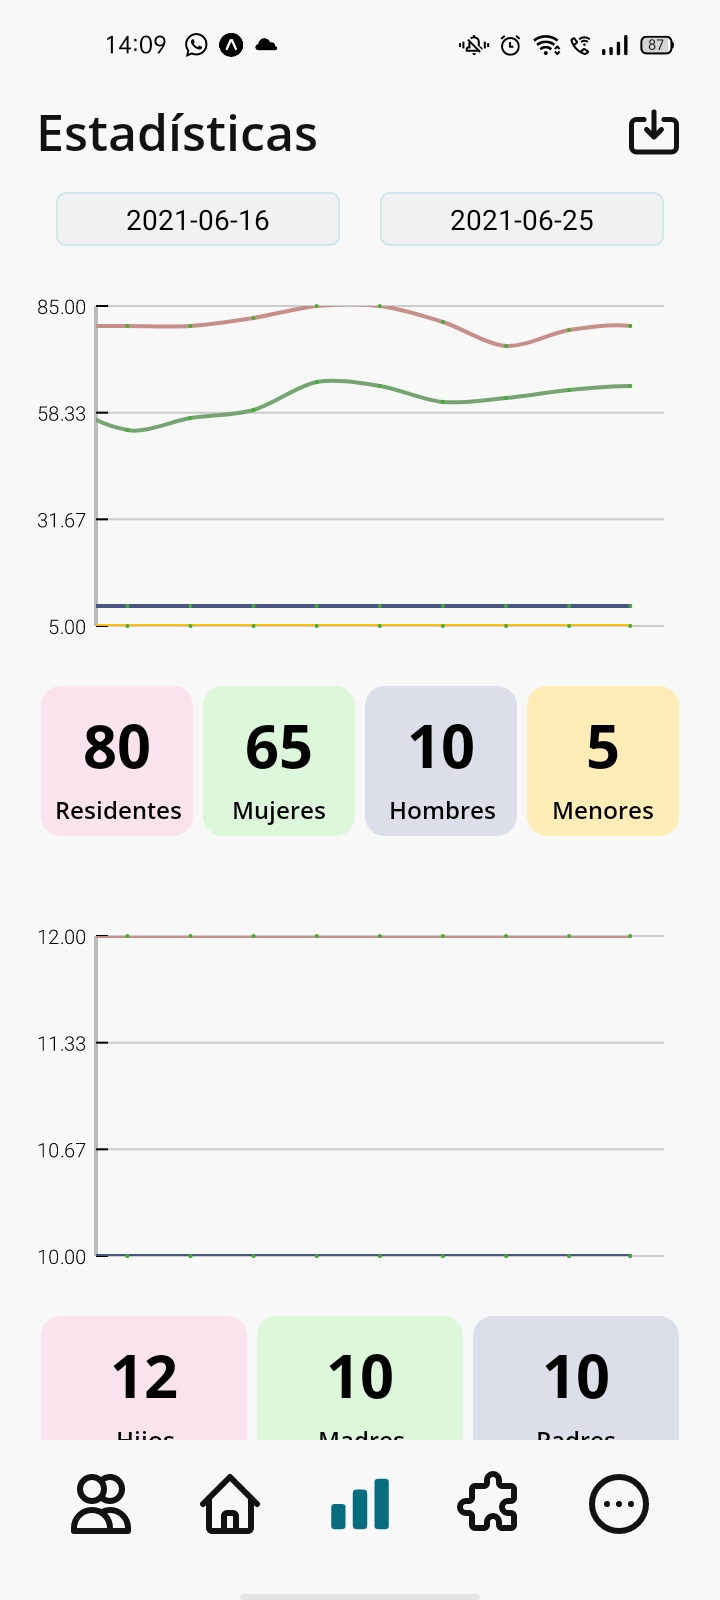
\includegraphics[width=0.30\linewidth]{imagenes/manual_usuario/estadisticas.jpg}
    \caption{Pantalla de casa (izquierda) y pantalla de estadísticas (derecha)}
    \label{fig:man-4}

\end{figure}

\subsection{Estadísticas}

Para la visualización de estadísticas tenemos la tercera sección de la aplicación (Figura \ref{fig:man-4}, derecha). En esta pantalla tendremos en la parte superior un botón con la función de exportar todos los datos de la aplicación. Para visualizar las estadísticas seleccionaremos un periodo de tiempo en la componente superior. Las estadísticas se mostrará en grupos de 4 para facilitar la visualización de los gráficos. Si pulsamos sobre alguno de los bloques, la gráfica pasará a mostrar ese único dato y ocultará los demás.

\subsection{Gestión de actividades}

La gestión de actividades está contemplada en la cuarta sección de la aplicación (Figura \ref{fig:man-5}, izquierda). Aquí nos mostrarán todas las actividades, separadas por las pasadas y las siguientes. Pulsando el botón superior podremos añadir una nueva actividad. Si pulsamos sobre alguna de ellas, nos llevará a la pantalla correspondiente a esta actividad (Figura \ref{fig:man-5}, centro). Esta contendrá la información correspondiente y sus acciones. En caso de que seamos asistentes, la única acción posible será la de apuntarse y desapuntarse a la actividad. En caso de que seamos administradores o usuarios generales, las acciones serán las de editar, eliminar y puntuar a los asistentes en el botón inferior. Si pulsamos este último, aparecerá un formulario con la puntuación actual de cada uno de los asistentes en una lista. Esta la podremos modificar.

\begin{figure}[h!]
    \centering
    
    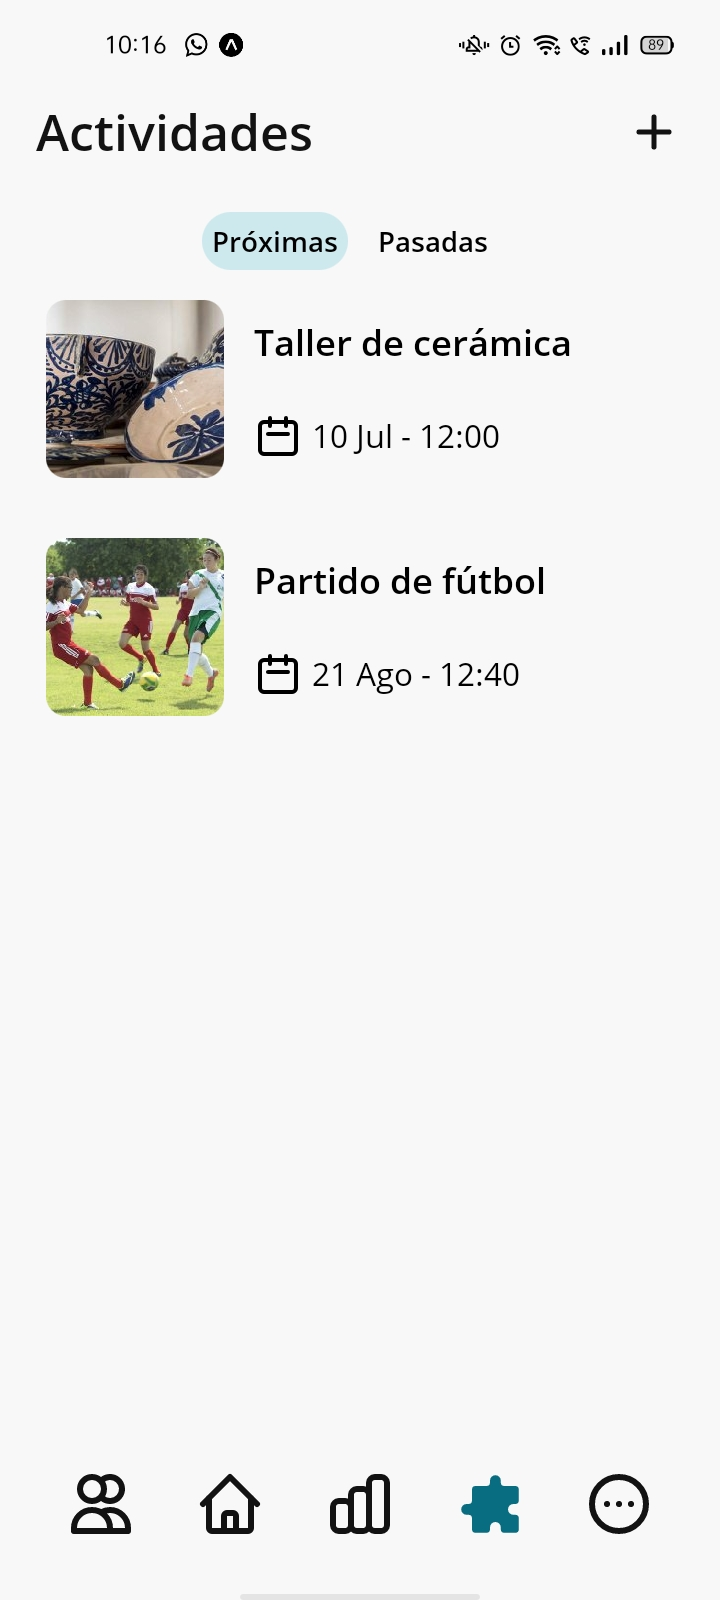
\includegraphics[width=0.30\linewidth]{imagenes/manual_usuario/actividades.jpg}
    \hspace{0.03\linewidth}
    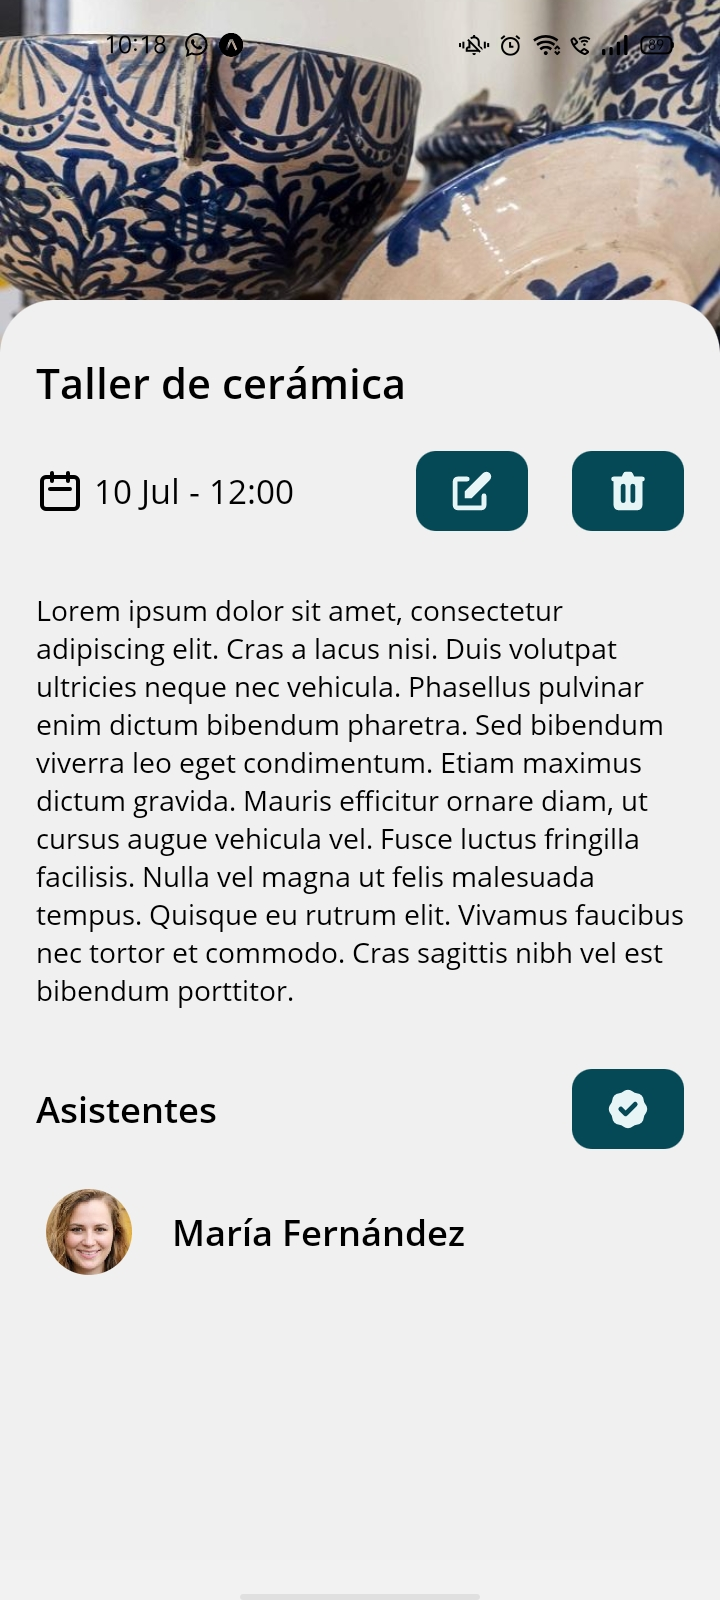
\includegraphics[width=0.30\linewidth]{imagenes/manual_usuario/actividad.jpg}
    \hspace{0.03\linewidth}
    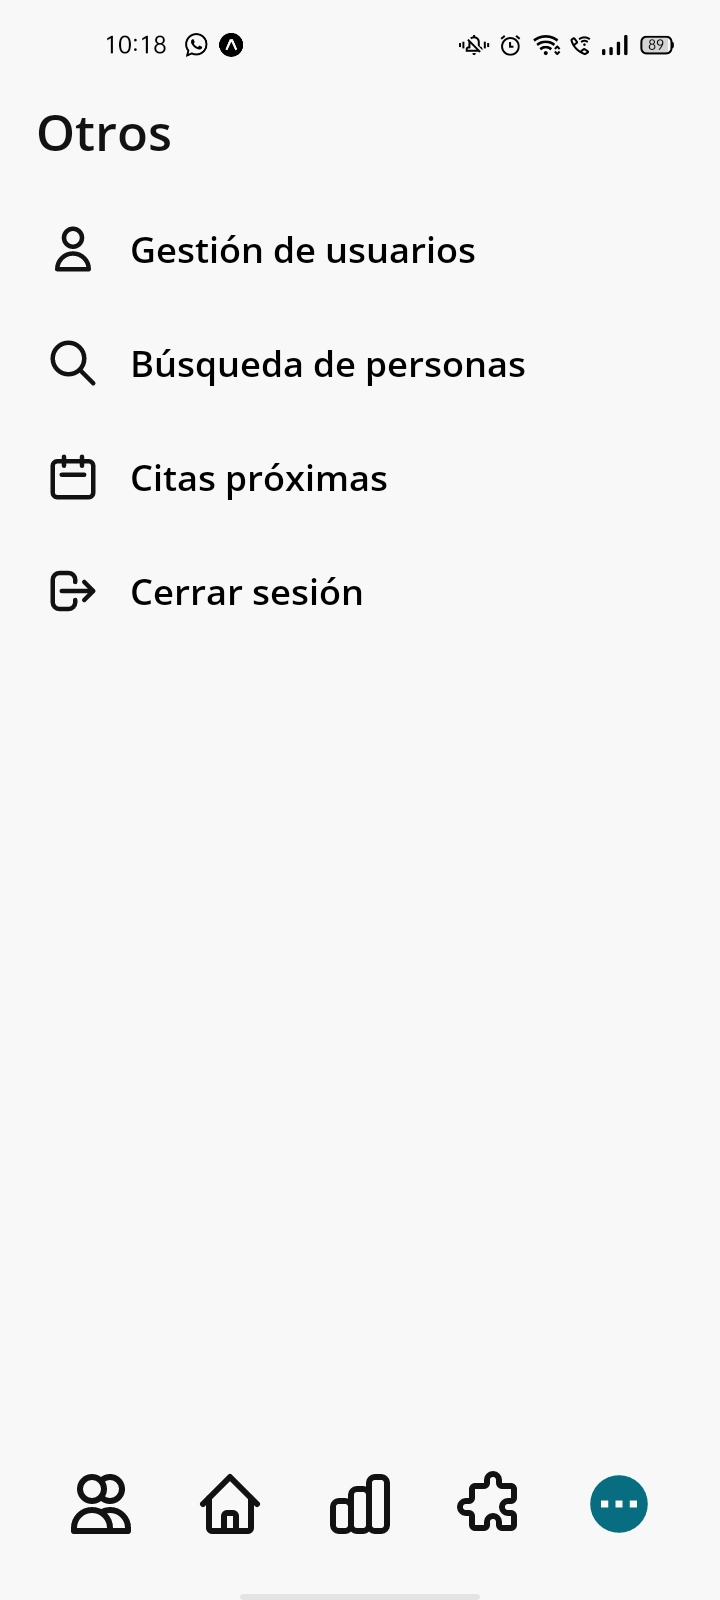
\includegraphics[width=0.30\linewidth]{imagenes/manual_usuario/acciones.jpg}
    \caption{Pantalla de actividades (izquierda), pantalla de actividad (centro) y pantalla de otras acciones (derecha)}
    \label{fig:man-5}

\end{figure}

En el caso de que seamos asistentes, en la pantalla de actividades, en lugar de aparecernos un botón para añadir una actividad, aparecerá un trofeo. Si lo pulsamos accederemos al ranking de usuarios y puntuación personal.

\subsection{Otras acciones}

La quinta sección contempla diferentes acciones menos usadas (Figura \ref{fig:man-5}, derecha). Una de las acciones de esta pantalla será la de cerrar la sesión lo que nos llevará al login.

\begin{figure}[h!]
    \centering
    
    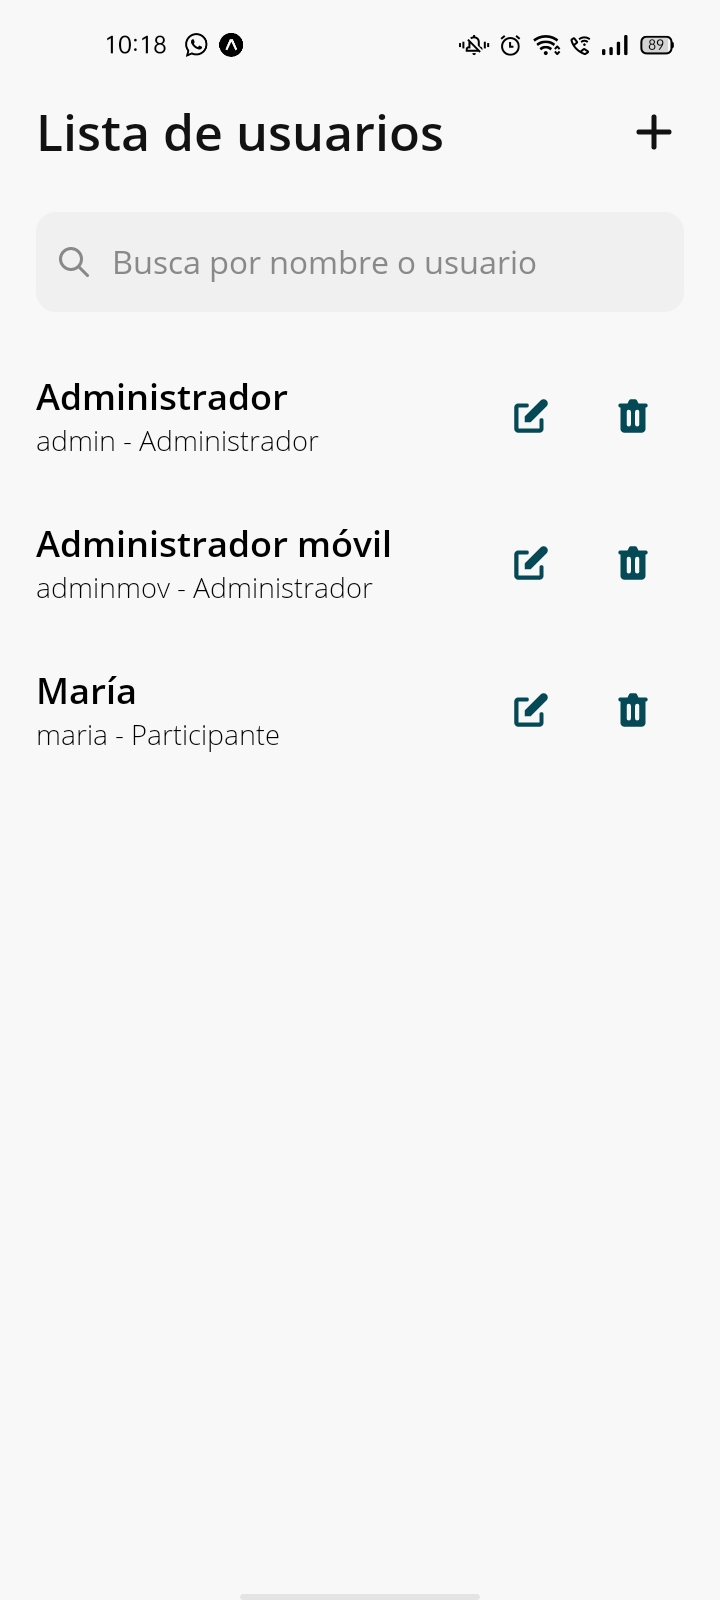
\includegraphics[width=0.30\linewidth]{imagenes/manual_usuario/usuarios.jpg}
    \hspace{0.03\linewidth}
    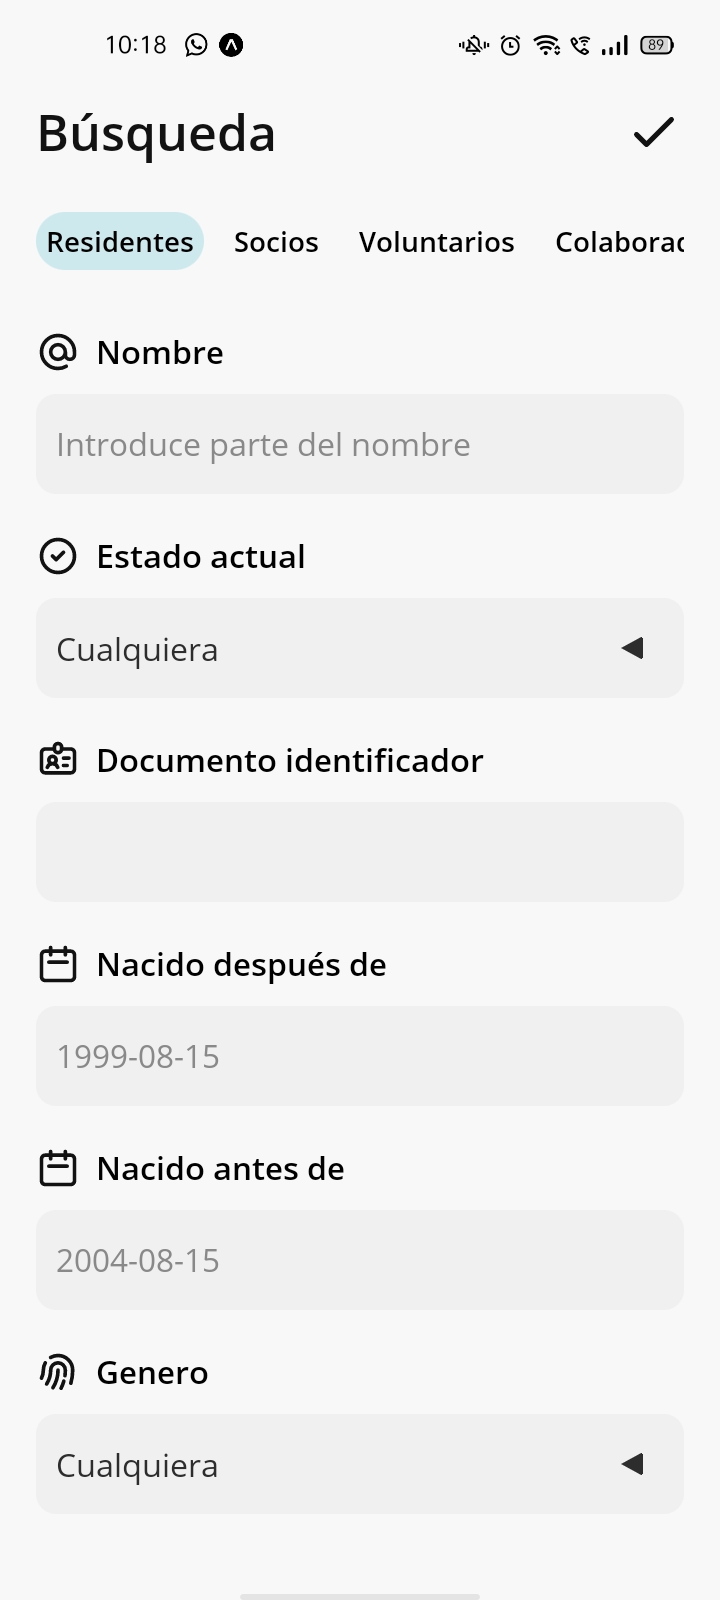
\includegraphics[width=0.30\linewidth]{imagenes/manual_usuario/busqueda.jpg}
    \hspace{0.03\linewidth}
    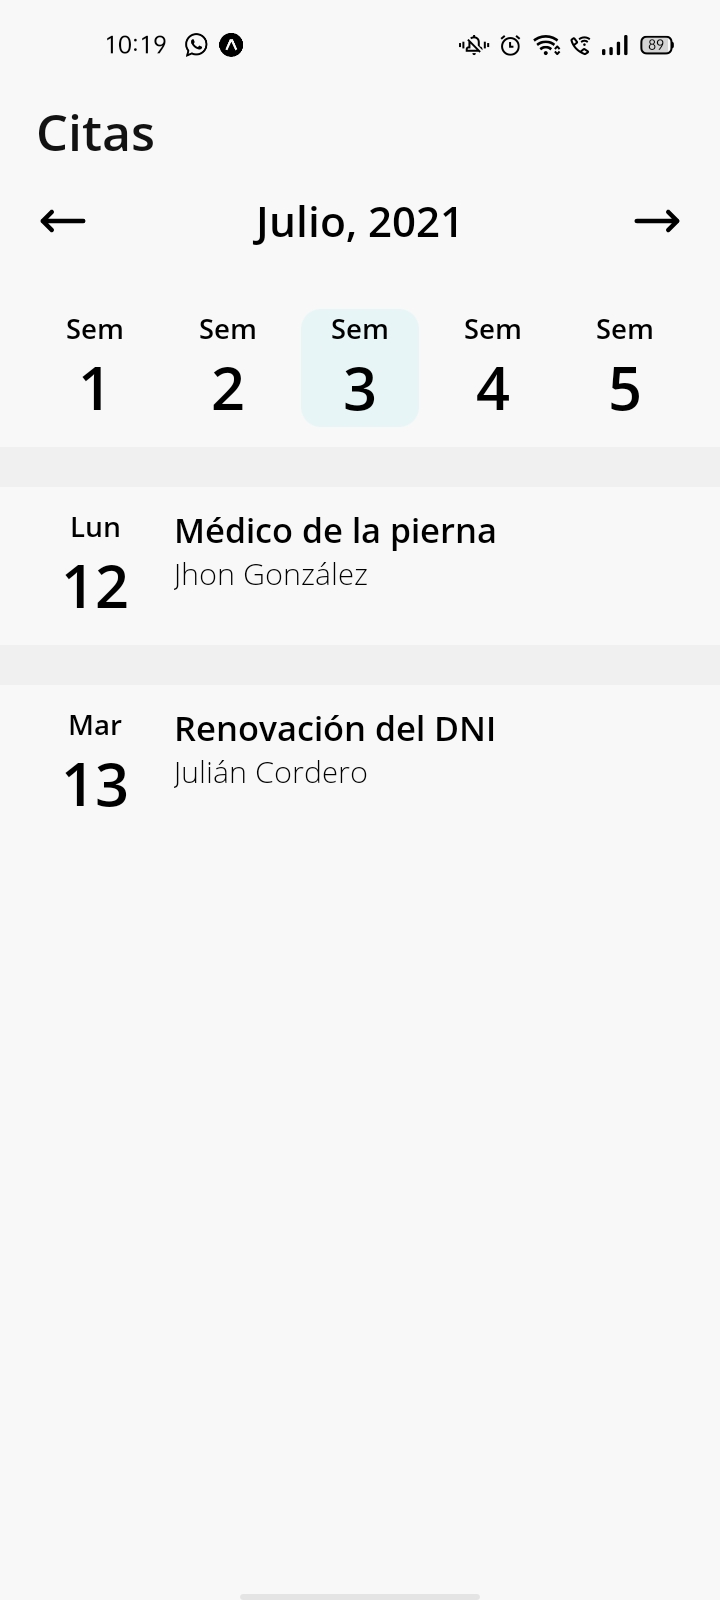
\includegraphics[width=0.30\linewidth]{imagenes/manual_usuario/citas.jpg}
    \caption{Pantalla de usuarios (izquierda), pantalla de búsqueda (centro) y pantalla de citas (derecha)}
    \label{fig:man-6}

\end{figure}

La primera opción de esta pantalla será la de gestionar los usuarios del sistema. Si entramos a esta, nos aparecerá una pantalla con la lista de usuarios del sistema (Figura \ref{fig:man-6}, izquierda), los cuales podremos editar y eliminar. Si pulsamos sobre el botón superior derecho, llegaremos a una pantalla la cual nos permitirá crear un usuario con sus diferentes parámetros. Esto ocurrirá de igual forma si decidimos editar un usuario.

La segunda sección será la de la búsqueda de personas (Figura \ref{fig:man-6}, centro). Aquí podremos añadir parámetros bajo los que se realizará una búsqueda de personas en el sistema.

La tercera opción será la de consultar las próximas citas (Figura \ref{fig:man-6}, derecha). Aquí nos aparecerá una pantalla en la cual podremos acceder a las citas de las personas ordenadas por semanas y meses.

